% ============================================================
% DIAGRAM: ADALINE / LMS (1960)
% ============================================================
% Caption: Figure 2.2: ADALINE architecture and LMS update.
%          (Adapted from Widrow & Hoff, 1960, p. 97)
% ============================================================

\documentclass[tikz,border=10pt]{standalone}
\usepackage{tikz}
\usepackage{amsmath}
\usepackage{amsfonts}

\usetikzlibrary{shapes,arrows,positioning,fit,calc,backgrounds}

\begin{document}

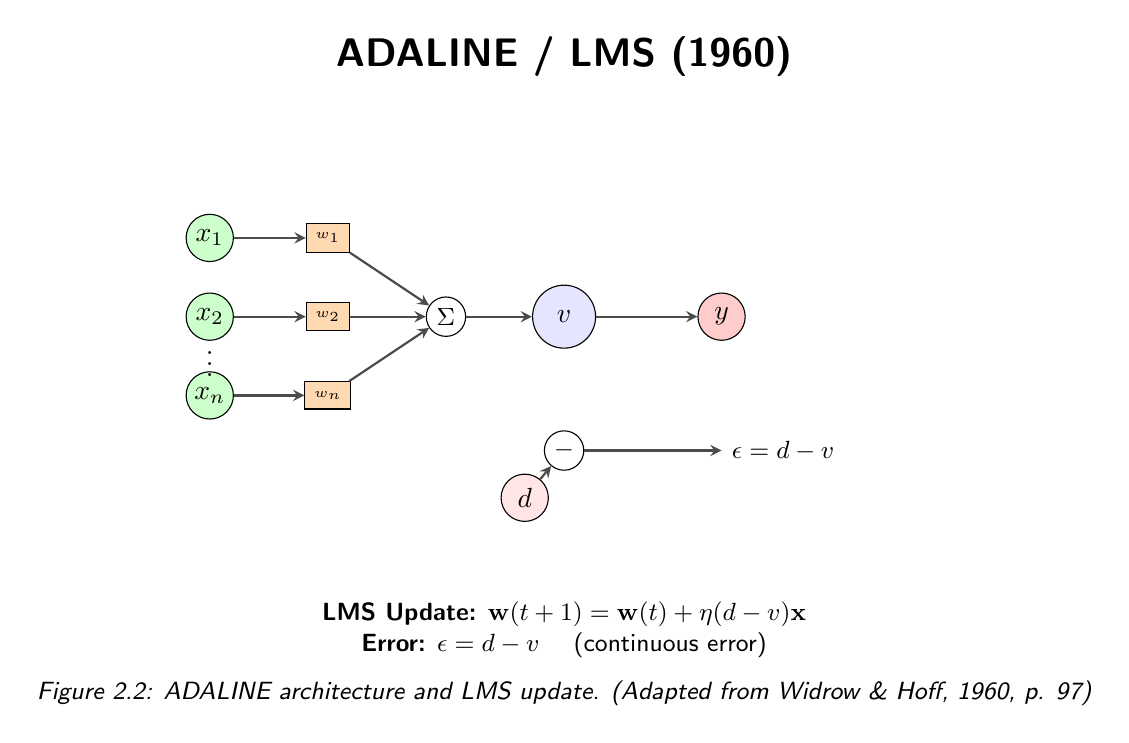
\begin{tikzpicture}[
    input/.style={draw, circle, minimum size=0.6cm, inner sep=0pt, fill=green!20},
    weight/.style={draw, rectangle, minimum width=0.5cm, minimum height=0.3cm, fill=orange!30, font=\tiny},
    sum/.style={draw, circle, minimum size=0.5cm, inner sep=0pt, fill=white, font=\sffamily\small},
    neuron/.style={draw, circle, minimum size=0.8cm, inner sep=0pt, fill=blue!20},
    output/.style={draw, circle, minimum size=0.6cm, inner sep=0pt, fill=red!20},
    label/.style={font=\sffamily\small},
    title/.style={font=\sffamily\Large\bfseries},
    caption/.style={font=\sffamily\small\itshape},
    edge/.style={-stealth, thick, draw=black!70},
]

\node[title] at (0, 3.8) {ADALINE / LMS (1960)};

% Inputs
\node[input] (x1) at (-4.5, 1.5) {$x_1$};
\node[input] (x2) at (-4.5, 0.5) {$x_2$};
\node[input] (xn) at (-4.5, -0.5) {$x_n$};
\node at (-4.5, 0) {$\vdots$};

% Weights
\node[weight] (w1) at (-3, 1.5) {$w_1$};
\node[weight] (w2) at (-3, 0.5) {$w_2$};
\node[weight] (wn) at (-3, -0.5) {$w_n$};

% Sum (linear combiner)
\node[sum] (sum) at (-1.5, 0.5) {$\Sigma$};

% Linear output
\node[neuron, fill=blue!10] (v) at (0, 0.5) {$v$};

% Quantizer
\node[output] (y) at (2, 0.5) {$y$};

% Error
\node[sum] (error) at (0, -1.2) {$-$};
\node[input, fill=red!10] (d) at (-0.5, -1.8) {$d$};
\draw[edge] (d) -- (error);
\draw[edge] (error) -- ++(2,0) node[right, font=\sffamily\small] {$\epsilon = d - v$};

% Edges
\draw[edge] (x1) -- (w1);
\draw[edge] (x2) -- (w2);
\draw[edge] (xn) -- (wn);
\draw[edge] (w1) -- (sum);
\draw[edge] (w2) -- (sum);
\draw[edge] (wn) -- (sum);
\draw[edge] (sum) -- (v);
\draw[edge] (v) -- (y);

% Equation
\node[align=center, font=\sffamily\small, anchor=north] at (0, -3.0) {
  \textbf{LMS Update:} $\mathbf{w}(t+1) = \mathbf{w}(t) + \eta (d - v) \mathbf{x}$ \\
  \textbf{Error:} $\epsilon = d - v$ \quad (continuous error)
};

\node[caption, anchor=north] at (0, -4.0) {
  Figure 2.2: ADALINE architecture and LMS update. (Adapted from Widrow \& Hoff, 1960, p. 97)
};

\end{tikzpicture}
\end{document}
